\section{Anropssignal}

Innehavare av ett amatörradiocertifikan eller amatörradiotillstånd ska
ha egen anropssignal. Enligt det internationella radioreglementet ska
anropssignalen för an amatörradiostation inledas med ett \emph{prefix}
som i princip är en landskod vilken består av en eller två bokstäver.
En av de två bokstäverna kan bytas mot en siffra.

Efter prefixet ska det komma en \emph{siffra} och därefter avslutas
signalen med ett \emph{suffix} som är person eööer stationskoden.

Exempel på anropssignaler: SM4UEI, SA0LAT, SK0UX.

Där SM är prefixet för sverige i den äldre standarden när televerket
utdelade signaler, 4 är distriktssiffran för dalarna och värmland, UEI
är den personliga anropssignalen.

För SA0LAT är det SA som är prefixet för sverige, 0 är
distriktssiffran för stockholmsområdet och LAT är den personliga
anropssignalen.

I den sista, SK0UX, så är landsprefixet SK för sverige, 0 för
stockholmsområdet och UX är stationskoden. Denna signal är en
radioklubbsignal, serien SK används bara för detta.

\section{Sveriges distrikt}

Sverige delas in i ett antal geografiska distrikt. Dessa distrikt ger
siffran mellan prefix och suffix i en anropssignal. Normalt används
den distriktsiffra där radioamatören är folkbokförd.

\begin{tabularx}{\columnwidth}{lX}
  \textbf{Distrikt} & \textbf{Område}\\ \hline
  0 & Stockholm\\
  1 & Gotland\\
  2 & Västerbotten, Norrbotten\\
  3 & Gävleborg, Västernorrland, Jämtland\\
  4 & Dalarna, Värmland\\
  5 & Uppsala, Södermanland, Östergötland, Västmanland\\
  6 & Halland, Västra Götaland\\
  7 & Jönköping, Kronoberg, Kalmar, Blekinge, Skåne\\
\end{tabularx}

\begin{figure}
  \centering
  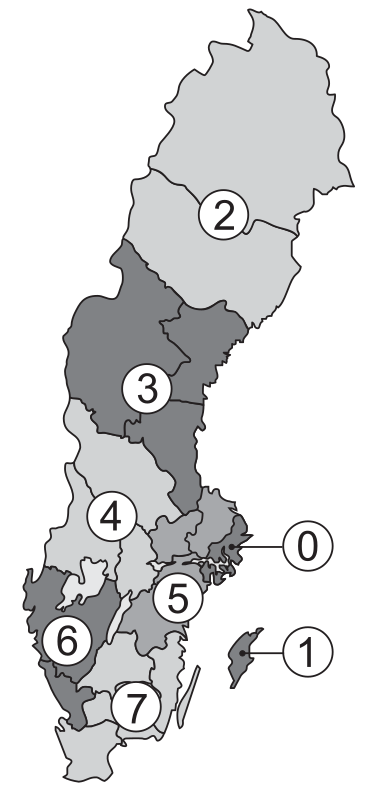
\includegraphics[width=.5\columnwidth]{blabok/pictures/R5-1.png}
\end{figure}

%Layout
\newpage

\section{Svenska prefix}

I Sverige finns flera olika prefix som kan användas. Nya radioamatörer
får alltid en signal med prefix SA. Äldre amatörer som avlade sitt
prov på den tiden televerket höll i provförrättningen fick signaler
med prefix SM. Dessa är de vanligaste prefixen som används.

Radioklubbar kan få signaler med prefix SA eller SK. Militära
amatörradiostationer och FRO (Frivilliga Radioorganisationen) får
signaler med prefixet SL.

För specialsignaler kan om det finns särskilda skäl för detta, t.ex.
för radiotävlingar och liknande ändamål, specialsignaler tilldelas.
Dessa tilldelas i någon av serierna 7S, 8S, SA, SB, SC, SD, SE, SF,
SG, SH, SI, SJ, SK, SL och SM.

%Layout
\newpage

\section{Anropssignaler}

\paragraph{Amatörradiosignalens utformning} \hfill \\

Tidigare har myndigheterna krävt att anropssignalen ska visa så
detaljerat som möjligt varifrån utsändningen äger rum. Detta krav
finns inte längre.

Praxis är numera att:

\begin{itemize}
\item Vid sändning från din ordinaria bostad
  (folkbokföringsadressen) används din vanliga anropssignal
  exempelvis SA0LAT.
\item Vi sändning från annan plats, t.ex. sommarbostad eller
  motsvarande visas detta genom att lägga till distriktsiffran där
  du befinner dig för tillfället, till exempel: SM0UE/4 eller SA0IPA/0, i det
  senare fallet sänder SA0IPA från en annan än ordinarie plats men
  i samma distrikt.
\item Har du däremot en fast fritidsadress kan tillägget
  utelämnas. Har du en sommarstuga i Värmland kan du i stället
  byta din ordinarie distriktsiffra till den siffra som gäller
  för distriktet, t.ex. SM0UEI byter till SM4UEI.
\item Tilläget /M visar att man är mobil. Mobil betyder
  radiosändare i alla former av rörelse. Anger man signalen
  SM0UEI/M är man mobil i sitt ordinarie distrikt. Är man i
  ett annat distrikt kan man lägga till distriktsiffran också
  och det kan då bli SM0UEI/3/M (tidigare angav man det som
  SM0UEI/3M men det fungerar inte bra med vissa loggprogram).
  
\item Befinner du dig i en båt på internationellt vatten kan
  du lägga till /MM (maritime mobile).
\item Vid sändning från flugplan används tillägge /AM
  (aeronautical mobile)
\end{itemize}

Det krävs normalt ett särskilt tillsånd att få sända från flygplan och
ges normalt inte för kommersiella flygplan.

Vid sändning från annat land som accepterat CEPT:s rekommendationer
som beskrivs i kapitel R8 ska amatörradiosignalen börja med landets
prefix, åtföljt av snedsteck och din anropssignal.

I de flesta fall är prefixet det som kallas landets identitetsprefix
men det kan finnas undantag.

\begin{itemize}
\item LA/SM0WKA innebär att amatören är i Norge
\item DL/SA0IPA innebär att amatören är i Tyskland
\item VE/SM0UEI innebär att amatören är i Kanada
\end{itemize}

En utländsk sändaramatör på besök i sverige får på motsvarande sätt
prefixet SA eller SM före den egna anropssignalen. Exempelvis får då
en sändaramatör från Finland anropssignalen SA/OH6ZR eller SM/OH0BKZ.

I tävlingssammanhang (contest) är det ibland nödvändigt att uppge i
vilket distrikt man befinner sig. Till exempel: SM3/OH6ZR.

Vid sändning från ett fartyg som är registrerat i annat land innebär
det att man befinner sig på det landets territorium även när fartyget
ligger vid kaj.

Amatörradiotillstånd gäller nprmaöt maximalt tre månader i annat land.
Stannar man längre, kan man åberopa den så kallade
HAREC-överenskommelsen och då får man ett tillstånd och en
anropssingal utfärdad i det landet (gäller endas i de länder som
tillämpar CEPT-rekommendationen T/R 61-02 HAREC).

Se KonCEPT för mer information om HAREC och de rekommendationer som
hör till detta.

\emph{Mer information om att sända frn annat land, oavsett om landet
  du ska besöka tillämpar CEPT-re\-kom\-men\-da\-tio\-n\-en eller inte, se SSA:s
  webbplats www.ssa.se under rubriken ``Att köra radio utomlands''.}

\section{Olika länders prefix}

Prefixen bestäms av Internationella Teleunionen. Varje land har
tilldelats 1-, 2- eller 3-ställiga prefix. Tidigare, när det inte fan
så många sändaramatörer använders i varje land endast ett prefix.

Detta prefix (i vissa fall två eller flera prefix) har blivit en
identitet för respektive land, även när andra prefix tillkommit. I
Sverige är denna identitet \textbf{SM}.

\textbf{Nordiska länder:}

\begin{tabular}{ll}
  LA, LB & Norge\\
  OH & Finland\\
  OHØ & Åland\\
  OZ & Danmark\\
\end{tabular}

\textbf{Europeiska länder:}

\begin{tabular}{ll}
  DL & Tyskland\\
  EA & Spanien\\
  ES & Estland\\
  F & Frankrike\\
  G, M & Storbrittannien\\
  HB & Schweiz\\
  I & Italien\\
  LY & Litauen\\
  OK & Tjeckien\\
  ON & Belgien\\
  PA & Holland\\
  S5 & Slovenien\\
  SP & Polen\\
  SV & Grekland\\
\end{tabular}

\textbf{Afrika och Asien:}

\begin{tabular}{ll}
  EA8 & Kanarieöarna\\
  ZS & Sydafrika\\
  HS & Thailand\\
  JA & Japan\\
\end{tabular}

\textbf{Amerikas och Oceanien:}
    
\begin{tabular}{ll}
  W, A, N, K & USA\\
  VE & Kanada\\
  LU & Argentina\\
  PY & Brasilien\\
  VK & Australien\\
  ZL & Nya Zeeland\\
\end{tabular}

%Layout
\newpage

\section{QSO på kortvåg}

Radiovågorna kan nå mycket långt på kortvåg, ibland så långt att man
kan tala direkt med andra sidan planeten. Det är också många som kan
avlyssna vad som sägs vid en kontakt på kortvåg jämfört med en kontakt
på UHF/VHF.

Det är viktigt att komma ihåg att använda ett vårdat språk samt att
följa de rutiner som är vanliga på kortvåg. Det är dessutom viktigt
att alla följer bandplanen så att det inte blir konflikter mellan
olika typer av radiotrafik.

De metoder som används för att genomföra en radiokontakt varierar
något beroende på bilket frekvensband som används och vilken typ av
radiotrafik som är aktuell. En kontakt på 14 MHz med en DX-expedition
skiljer sig givetvis från en lokal kontakt på HF, VHF eller UHF.

\section{Anrop}

Innan ett allmänt anrop görs kontrollerar man alltid om frekvensen är
upptagen. Ett allmänt anrop skall vara tydligt och kort. Det är bättre
att göra flera korta anrop med intervaller än att hålla långa anrop.

Vid anrop anger man alltid motstationens anropssignal först, därefter
sin egen.

\section{Identifiering}

Sändar- och mottagarstationes anropssignal skall användas i början och
i slutet av varje förbindelse. Under förbindelsen ska anropssignalen
upprepas med korta mellanrum. Vid identifiering skall den egna
anropssignalen \emph{alltid sändas sist}.

Bokstavera sådant som är svårt att uppfatta som anropssignaler, namn
och QTH (din plats).

%Layout
\newpage

\section{Trafikexempel}

\textit{Kontrollera om frekvensen är upptagen:}

\textbf{Är denna frekvens upptagen?}

\textit{Eller på engelska}

\textbf{Is this frequency in use?}
  
\textit{Allmänt anrop på svenska eller engelska:}

\textbf{Allmänt anrop, allmänt anrop, allmänt anrop från SAØLAT,
  SAØLAT, SAØLAT, kom.}

\textbf{CQ CQ CQ this is SAØIPA SAØIPA SAØIPA calling CQ and
  listening}

Och för telegrafi kan man sända exempelvis:

\textbf{CQ CQ CQ DE SMØUEI SMØUEI SMØUEI K}

Ett svar på det allmänna anropet ser oftast ut som ett vanligt anrop
tillbaka:

\textbf{SAØIPA från SAØLAT SAØLAT SAØLAT, kom.}

Vanligast är att man bokstaverar anropssignalerna.

Ett engelskt svar kan se ut såhär:

\textbf{SA3BYC from GØVDJ GØVDJ GØVDJ, calling you and listening}

Och i telegrafi och digitala trafiksätt:

\textbf{SM4ABC DE SM5XYZ SM5XYZ SM5XYZ K}

\vspace{1em} \hrule \vspace{1em}

\emph{Kom ihåg:}

\begin{itemize}
  \item En anropssignal består av ett landsprefix, en siffra och ett
    suffix
  \item Vid anrop ska alltid motstationens anropssignal anges först

  \item Kontrollera alltid om frekvensen är upptagen innan ett
    allmänt anrop görs
    
  \item Använd vårdat språk -- alltid
\end{itemize}

\emph{Lär dig:}

\begin{itemize}
\item Amatörradiosignalens utformning
\item Hur olika länders prefix ser ut
\item Hur ett allmänt anrop går till
\item Hur ett svar på ett anrop går till
\end{itemize}
